\section[Description du mouvement d'un point matériel]{Description du mouvement d'un point\\matériel par rapport à deux référentiels mobiles l'un par rapport à l'autre}

    \subsection{Mouvement d'un référentiel par rapport à l'autre}

        \subsubsection{Translation}

            On considère $\mathcal{R}(Oxyz)$ et $\mathcal{R}'(O'x'y'z')$ (trièdres orthonormés directs pour simplifier).

            \begin{definition}[Référentiel en translation par rapport à un autre]
                $\mathcal{R}'$ est en translation par rapport à $\mathcal{R}$ si ses axes gardent une orientation constante par rapport aux axes du référentiel $\mathcal{R}$.
            \end{definition}

            Il y a donc une seule inconnue : $\vec{OO'}(t)$.

            \begin{example}
                Le référentiel géocentrique (origine au centre de la Terre et trois axes pointés vers trois étoiles lointaines \og fixes\fg) est (environ) en translation circulaire par rapport au référentiel de Copernic (origine au centre du système solaire et trois axes pointant vers trois étoiles \og fixes\fg), voir la Figure~\ref{fig:refentiel_geocentrique_copernic}.
                \begin{figure}[!h]
                    \centering
                    \tikzsetnextfilename{refentiel_geocentrique_copernic}
                    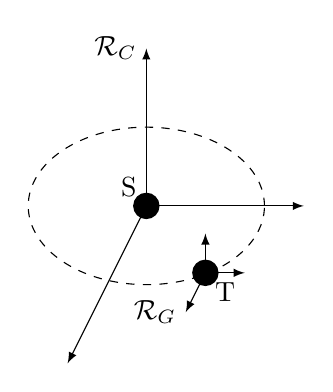
\begin{tikzpicture}[scale=1]  
                        % \helpgrid{3}{3}
                        \coordinate (S) at (0,0); \node at (S) [above left] {S};
                        \draw [->,-latex] (S) --++ (-1,-2)	;   
                        \draw [->,-latex] (S) --++ (2,0);
                        \draw [->,-latex] (S) --++ (0,2) node [left] {$\mathcal{R}_C$}	; 
                        \draw [line width=1pt,fill=black] (S) circle (0.15cm); 
                        \draw [dashed] (S) ellipse (1.5cm and 1cm);
                        \coordinate (T) at (0.75,-0.85); \node at (T) [below right] {T};
                        \draw [line width=1pt,fill=black] (T) circle (0.15cm);                
                        \draw [->,-latex] (T) --++ (-0.25,-0.5)	node [left] {$\mathcal{R}_G$};   
                        \draw [->,-latex] (T) --++ (0.5,0);
                        \draw [->,-latex] (T) --++ (0,0.5) 	;
                    \end{tikzpicture}
                    \caption{Référentiel géocentrique et de Copernic.}    
                    \label{fig:refentiel_geocentrique_copernic}
                \end{figure}
            \end{example}

        \subsubsection{Rotation uniforme autour d'un axe fixe}
            
            \begin{example}
                La rotation propre de la Terre (référentiel $\mathcal{R}_{T}$) par rapport à l'axe reliant ses pôles, de vitesse angulaire $\omega=\dot{\theta}$ par rapport à l'axe de rotation (supposé selon l'axe $z$). On note alors le vecteur de rotation instantanée
                \begin{equation*}
                    \vec{\omega}(\mathcal{R}_{T}/\mathcal{R}_{G})\coloneqq \dot{\theta}\,\vec{u_z},
                \end{equation*}
                où $\mathcal{R}_{G}$ est le référentiel géocentrique, $\dot{\theta}$ est la vitesse angulaire de rotation et $\vec{u_z}$ donne la direction et le sens de rotation.
            \end{example}

    \subsection{Dérivée d'un vecteur exprimée dans deux référentiels en mouvement relatif}

        Soit $\mathcal{R}(Oxyz)$ et $\mathcal{R}'(O'x'y'z')$ et $\vec{A}$ quelconque. On se demande quelle est la relation entre $\left(\dfrac{\d\vec{A}}{\d t}\right)_{\mathcal{R}}$ et $\left(\dfrac{\d\vec{A}}{\d t}\right)_{\mathcal{R}'}$. Pour cela, projetons $\vec{A}$ sur les vecteurs de base de $\mathcal{R}'(\vec{u_x}',\vec{u_y}',\vec{u_z}')$:
        \begin{equation*}
            \vec{A}(t) = a(t)\vec{u_x}'+b(t)\vec{u_y}'+c(t)\vec{u_z}'.
        \end{equation*}

        \begin{itemize}
            \item Dans $\mathcal{R}'$, comme $(\vec{u_x}',\vec{u_y}',\vec{u_z}')$ est une base fixe dans $\mathcal{R}'$, on a 
            \begin{equation*}
                \left(\frac{\d\vec{A}}{\d t}\right)_{\mathcal{R}'}=\dfrac{\d a}{\d t}\vec{u_x}'+\dfrac{\d b}{\d t}\vec{u_y}'+\dfrac{\d c}{\d t}\vec{u_z}'.
            \end{equation*}
            \item Dans $\mathcal{R}$, on a 
            \begin{align*}
                \left(\frac{\d\vec{A}}{\d t}\right)_{\mathcal{R}}
                &=\frac{\d a}{\d t}\vec{u_x}'+\frac{\d b}{\d t}\vec{u_y}'+\frac{\d c}{\d t}\vec{u_z}'\\
                &\quad+a(t)\left(\frac{\d\vec{u_x}'}{\d t}\right)_{\mathcal{R}}+b(t)\left(\frac{\d\vec{u_y}'}{\d t}\right)_{\mathcal{R}}+c(t)\left(\frac{\d\vec{u_z}'}{\d t}\right)_{\mathcal{R}}.
            \end{align*}
        \end{itemize}
        Si $\mathcal{R}'$ est en translation par rapport à $\mathcal{R}$, alors $(\vec{u_x}',\vec{u_y}',\vec{u_z}')$ est fixe dans $\mathcal{R}$ et ainsi 
        \begin{equation*}
            \left(\dfrac{\d\vec{A}}{\d t}\right)_{\mathcal{R}}=\left(\dfrac{\d\vec{A}}{\d t}\right)_{\mathcal{R}'}.
        \end{equation*}
        Si $\mathcal{R}'$ est en rotation uniforme par rapport à l'axe $(Oz)$, on décompose les vecteurs de base :
        \begin{equation*}
            \left\lbrace
            \begin{aligned}
                \vec{u_x}' &= \cos\theta\vec{u_x}+\sin\theta\vec{u_y},\\
                \vec{u_y}' &= -\sin\theta\vec{u_x}+\cos\theta\vec{u_y},\\
                \vec{u_z}' &= \vec{u_z}.
            \end{aligned}
            \right.
        \end{equation*}
        Alors on a 
        \begin{equation*}
            \begin{aligned}
                \left(\frac{\d\vec{u_x}'}{\d t}\right)_{\mathcal{R}} &= -\dot{\theta}\sin\theta\,\vec{u_x}+\dot{\theta}\cos\theta\,\vec{u_y}=\dot{\theta}\,\vec{u_y}'=\dot{\theta}\left(\vec{u_z}\wedge\vec{u_x}'\right),\\
                \left(\frac{\d\vec{u_y}'}{\d t}\right)_{\mathcal{R}} &= -\dot{\theta}\cos\theta\,\vec{u_x}-\dot{\theta}\sin\theta\,\vec{u_y}=-\dot{\theta}\,\vec{u_x}'=\dot{\theta}\left(\vec{u_z}\wedge\vec{u_y}'\right).
            \end{aligned}
        \end{equation*}
        Or $\vec{\omega}(\mathcal{R}'/\mathcal{R})\coloneqq\dot{\theta}\,\vec{u_z}$, on écrit donc simplement
        \begin{equation*}
            \begin{aligned}
                \left(\frac{\d\vec{u_x}'}{\d t}\right)_{\mathcal{R}} &=\vec{\omega}\wedge\vec{u_x}',\\
                \left(\frac{\d\vec{u_y}'}{\d t}\right)_{\mathcal{R}} &=\vec{\omega}\wedge\vec{u_y}'.
            \end{aligned}
        \end{equation*}
        Ainsi,
        \begin{equation*}
            \left(\frac{\d\vec{A}}{\d t}\right)_{\mathcal{R}}=\left(\frac{\d\vec{A}}{\d t}\right)_{\mathcal{R}'}+\vec{\omega}\wedge(a\vec{u_x}'+b\vec{u_y}'+c\vec{u_z}').
        \end{equation*}
        De manière générale, on a donc 
        \begin{equation*}
            \boxed{
                \left(\frac{\d\vec{A}}{\d t}\right)_{\mathcal{R}}=\left(\frac{\d\vec{A}}{\d t}\right)_{\mathcal{R}'}+\vec{\omega}(\mathcal{R}'/\mathcal{R})\wedge\vec{A}.
            }
        \end{equation*}
    
    \subsection{Composition des vitesses et vitesse d'entraînement}
        \subsubsection{Translation}

            Soit $M$ un point matériel et $\mathcal{R}'(O'x'y'z')$ un référentiel en translation par rapport à un autre référentiel $\mathcal{R}(Oxyz)$. La vitesse de $M$ dans le référentiel $\mathcal{R}$ est
            \begin{equation*}
                \vec{v}(M)_{/\mathcal{R}}\coloneqq\left(\frac{\d\vec{OM}}{\d t}\right)_{\mathcal{R}}=\underbrace{\left(\frac{\d \vec{OO'}}{\d t}\right)_{\mathcal{R}}}_{\vec{v}(O')_{/\mathcal{R}}}+\underbrace{\left(\frac{\d\vec{O'M}}{\d t}\right)_{\mathcal{R}}}_{\vec{v}(M)_{/\mathcal{R}'}}.
            \end{equation*}
            \begin{definition}[Vitesse d'entraînement]
                $\vec{v}_e\coloneqq\vec{v}(O')_{/\mathcal{R}}$ est appelée la \textbf{vitesse d'entraînement}, qui est indépendante de n'importe quel point matériel considéré, mais vient juste du fait que $\mathcal{R}'$ est en translation par rapport à $\mathcal{R}$.
            \end{definition}
            On a donc
            \begin{equation*}
                \boxed{
                    \vec{v}(M)_{/\mathcal{R}}=\vec{v}(M)_{/\mathcal{R}'}+\vec{v}_e.
                }
            \end{equation*}

            \paragraph{Mouvement de translation rectiligne uniforme.} On considère qu'à $t=0$, $O=O'$ et que le référentiel $\mathcal{R}'$ est en translation rectiligne uniforme à la vitesse $V$ selon l'axe $(Ox)$. \begin{itemize}
                \item Dans le cas non relativiste $v\ll c$, on a 
                \begin{equation*}
                    \frac{\d x}{\d t}=\frac{\d x'}{\d t}+V,
                \end{equation*}
                d'où $x=x'+Vt$ : c'est une transformation de Galilée. Comme on a $y=y'$, $z=z'$ et $t=t'$, on a 
                \begin{equation*}
                    \begin{pmatrix}
                        x\\y\\z\\t
                    \end{pmatrix}=\begin{pmatrix}
                        1&0&0&V\\0&1&0&0\\0&0&1&0\\0&0&0&1
                    \end{pmatrix}\begin{pmatrix}
                        x'\\y'\\z'\\t'
                    \end{pmatrix}.
                \end{equation*}

                \item Dans le cas relativiste $v\lessapprox c$, c'est la transformation de Poincaré-Lorentz :
                \begin{equation*}
                    \begin{pmatrix}
                        x\\y\\z\\xt
                    \end{pmatrix}=\begin{pmatrix}
                        \gamma&0&0&\beta\gamma\\
                        0&1&0&0\\
                        0&0&1&0\\
                        \beta\gamma&0&0&\gamma
                    \end{pmatrix}\begin{pmatrix}
                        x'\\y'\\z'\\ct'
                    \end{pmatrix},
                \end{equation*}
                où $\beta\coloneqq\frac{v}{c}\lessapprox1$ et $\gamma\coloneqq\dfrac{1}{\sqrt{1-\beta^{2}}}>1$.
                \begin{itemize}[label=$\longrightarrow$]
                    \item Dans la limite $\beta\ll1$, on a $\gamma\approx1$ et on retrouve la transformation de Galilée.
                    \item Le temps n'est plus absolu.
                    \item Il y a une \og dilatation\fg~des temps. En effet, soit un intervalle de temps propre dans $\mathcal{R}'$ (i.e.~séparant deux évènements ayant lieu au même endroit dans $\mathcal{R}'$). Alors 
                    \begin{equation*}
                        c\Delta t=\beta\gamma\underbrace{\Delta x'}_{=0}+\gamma c\Delta t'=\gamma c\Delta t'.
                    \end{equation*}
                    Ainsi, si $\Delta x=0$, $\Delta t$ est \og impropre\fg. On note que dans ce cas, $\Delta t_{\text{impropre}}=\gamma\Delta t_{\text{propre}}$ (et $\gamma>1$ donc il y a une \og dilatation\fg).
                \end{itemize}
            \end{itemize}

        \subsubsection{Rotation uniforme autour d'un axe fixe}

            On note $\vec{\omega}(\mathcal{R}'/\mathcal{R})=\dot{\theta}\vec{u_z}$. On a déjà vu que l'on a 
            \begin{equation*}
                \vec{v}(M)_{/\mathcal{R}}=\vec{v}(M)_{/\mathcal{R}'}+\vec{v}_e(M),
            \end{equation*}
            avec $\vec{v}_e(M)=\vec{\omega}(\mathcal{R}'/\mathcal{R})\wedge\vec{OM}$.

            Pour simplifier, on notera $\vec{v'}$ quand la vitesse sera calculée par rapport au référentiel $\mathcal{R}'$, et $\vec{v}$ quand la vitesse sera calculée par rapport au référentiel $\mathcal{R}$ (ce qui sera le cas par défaut).

    \subsection{Composition des accélérations}

        \subsubsection{Translation}

            On a
            \begin{equation*}
                \vec{a}(M)_{/\mathcal{R}}=\left(\dfrac{\d\vec{v}(M)}{\d t}\right)_{/\mathcal{R}}=
                \underbrace{\left(\frac{\d\vec{v}'}{\d t}\right)_{\mathcal{R}}}_{\left(\frac{\d\vec{v}'}{\d t}\right)_{\mathcal{R}'}+\vec{0}\coloneqq\vec{a'}(M)_{/\mathcal{R}'}}
                +\underbrace{\left(\frac{\d\vec{v}_e}{\d t}\right)_{\mathcal{R}}}_{\vec{a}_e}.
            \end{equation*}

            Ainsi,
            \begin{equation*}
                \boxed{
                    \vec{a}(M)=\vec{a'}(M)+\vec{a}_e,
                }
            \end{equation*}
            où $\vec{a}_e=\dfrac{\d^{2}\vec{OO'}}{\d t^{2}}$.

        \subsubsection{Rotation uniforme}

            On a 
            \begin{align*}
                \vec{a}(M)_{/\mathcal{R}}=\left(\frac{\d\vec{v}(M)}{\d t}\right)_{\mathcal{R}}
                &=\left(\frac{\d\vec{v'}}{\d t}\right)_{\mathcal{R}}+\left(\frac{\d}{\d t}\left(\vec{\omega}\wedge\vec{OM}\right)\right)_{\mathcal{R}},\\
                &=\left(\frac{\d\vec{v}}{\d t}\right)_{\mathcal{R}'}+\vec{\omega}\wedge\vec{v'}+\vec{\omega}\wedge\left(\frac{\d\vec{OM}}{\d t}\right)_{\mathcal{R}},
            \end{align*}
            où l'on a utilisé le fait que $\vec{\omega}$ est une constante. Comme 
            \begin{equation*}
                \left(\dfrac{\d\vec{OM}}{\d t}\right)_{\mathcal{R}}=\vec{v}(M)=\vec{v'}+\vec{\omega}\wedge\vec{OM},
            \end{equation*}
            on a donc 
            \begin{equation*}
                \boxed{
                    \vec{a}(M)_{/\mathcal{R}}=\vec{a}(M)_{/\mathcal{R}'}+\vec{\omega}\wedge\left(\vec{\omega}\wedge\vec{OM}\right)+2\vec{\omega}\wedge\vec{v'}.
                }
            \end{equation*}

            On note alors $\vec{a}_e(M)=\vec{\omega}\wedge\left(\vec{\omega}\wedge\vec{OM}\right)$ et $\vec{a}_c(M)=\vec{\omega}\wedge\vec{v'}$ \textbf{l'accélération de Coriolis}.

            \begin{example}
                Dans le cas d'une rotation autour de l'axe $(Oz)$, on a 
                \begin{equation*}
                    \begin{pmatrix}
                        0\\0\\\omega
                    \end{pmatrix}\wedge\begin{pmatrix}
                        x\\y\\z
                    \end{pmatrix}=\begin{pmatrix}
                        -\omega y\\\omega x\\0
                    \end{pmatrix},
                \end{equation*}
                puis
                \begin{equation*}
                    \begin{pmatrix}
                        0\\0\\\omega
                    \end{pmatrix}\wedge\begin{pmatrix}
                        -\omega y\\\omega x\\0
                    \end{pmatrix}=\begin{pmatrix}
                        -\omega^{2}x\\-\omega^{2}y\\0
                    \end{pmatrix}=-\omega^{2}\begin{pmatrix}
                        x\\y\\z
                    \end{pmatrix}.
                \end{equation*}
                Donc $\vec{a}_e(M)=-\omega^{2}\vec{HM}$ où $H$ est le projeté orthogonal sur l'axe $(Oz)$ du point $M$.
            \end{example}
